\section{Falcon工具的技术分析与重构}
\subsection{Falcon框架}
在图\ref{pic:falconFrame}中显示的是Falcon文件组织框架。在src/目录下是源代码,而src-dummy/,目录下是需要插装的方法的签名\footnote{方法的签名是方法声明的一部分,包括方法名和参数列表。}。
\begin{figure}[!ht]
  \centering
  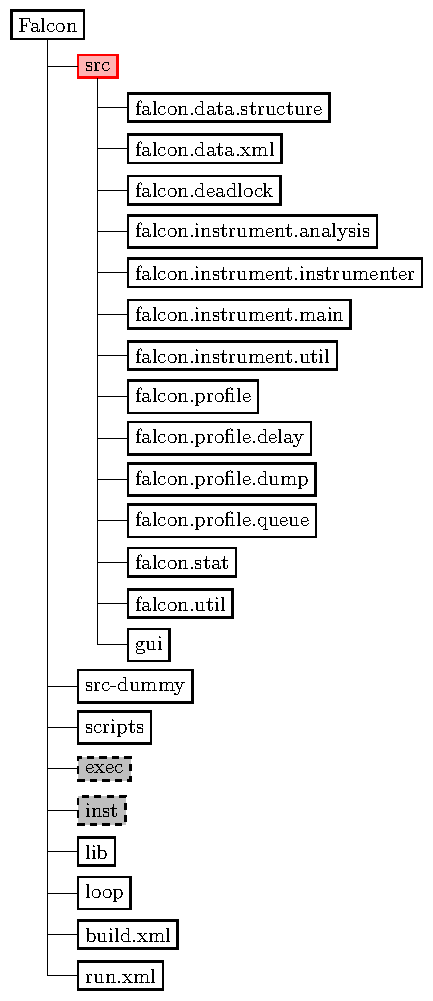
\includegraphics[width=.5\textwidth]{FileTree.pdf}
  \caption{Falcon文件组织框架}\label{pic:falconFrame}
\end{figure}
具体到src/目录里,falcon.data.structure里是Falcon中用到的数据结构。falcon.data.xml用来实现序列化和反序列化。falcon.deadlock 里的代码用于检测被测程序运行时是否死锁,如果死锁,execInfo里记录的运行结果将是Deadlock。falcon.instrument 里的代码用于实现插装。falcon.profile 里的代码主要是探针,用来插入到被测程序当中。
falcon.stat 里的代码用于统计结果,得到每一个模式的可疑度。falcon.util里的代码是Falcon中常用的数据类型。gui中的代码用于实现可视化。\par
scripts/下是Python脚本,用来自动化插装、运行多个被测程序。lib/下存放有Falcon中使用的类库。loop/有1.loop,10.loop,100.loop等文件,用来控制被测程序重复执行。build.xml和run.xml分别是使用ant进行编译和运行被测程序时的脚本。除了代码之外,还有inst和exec两个文件夹是运行Falcon过程中生成的,用来保存被测程序的插装结果和运行结果。\par
\subsection{被测程序的插装技术}
程序插装是指使被测试程序在保持原有逻辑完整性基础上在程序中插入一些探针,通过探针的执行并抛出程序的运行特征数据。基于这些特征数据分析,可以获得程序的控制流及数据流信息,进而得到逻辑覆盖等动态信息\cite{Instrument}。\par
实现插装时,Falcon使用Soot对被测程序进行静态的线程逃逸分析,从而确定一个变量是否被多个线程共享访问。如果一个变量是被多个线程访问,则插装该变量的读写操作,这样在程序运行时就可以得到访问共享变量的记录。如代码\ref{lst:inst}所示,对于一个Java语句``x = y + 1;'',在其前后分别进行插装探针,可以获得读变量y和写变量x的信息。
\begin{code}[language={[AspectJ]Java}, label=lst:inst, caption=插装程序读写操作示意]
  ...
  accessObj(method, Stmt(x=y+1), Var(y), read);
  x = y + 1;
  accessObj(method, Stmt(x=y+1), Var(x), write);
  ...
\end{code}
\subsubsection{线程逃逸分析}
在多线程程序当中,线程本地数据(thread local data)是指被一个线程拥有的数据。这里的``拥有''的意思是这些数据只能被这个线程访问\cite{threadlocal}。与之相对的是可以被多个线程访问的线程共享数据(thread shared data)。多个线程访问同一个数据可能会带来数据争用或死锁等问题。线程逃逸分析(thread escape analysis)的作用是监视所有对线程本地数据的访问,当检测到有另外一个线程尝试访问这个线程本地数据,即标记这个数据为逃逸(escaping)\cite{threadescape}。在Falcon中,首先需要通过线程逃逸分析判断一个变量是否被多个线程访问。
\subsubsection{Soot简介}
Soot是加拿大McGill大学Sable研究组开发的Java字节码分析和优化开源工具。它为字节码的分析、优化、反编译、注解等提供一个可扩展的框架\cite{jnuthesis2}。Soot作为字节码分析和转换工具,广泛地应用于编译器优化研究,程序分析等领域中。\par
Soot在Falcon工具中主要有三个作用。一是对被测程序进行静态的线程逃逸分析,用来确定一个变量是否被多个线程访问。在Soot的soot.jimple.toolkits.thread.ThreadLocalObjectsAnalysis包中提供了相应的API可以用来进行线程逃逸分
析\cite{halpert2008static}。二是使用Soot分析Java语句来判断线程对变量的访问是读还是写。三是使用Soot提供的API将探针插装到被测程序当中。
\subsubsection{插装的过程}\label{sec:InstProcess}
Soot的分析与变化是建立在其内部的中间表示法(Intermediate Representation,IR)上\cite{jnuthesis1}。 在Falcon中,使用的IR 是Jimple---Soot 中最核心的IR。在Soot里可以按照需要对Jimple进行分析、变换和优化,并生成相应.class文件。在Falcon进行插装时,需要运行falcon.instrument.main.Main.java。该类继承SceneTransformer类,重写了\texttt{internalTransformer()}方法,可以将探针插装到Jimple中间表示当中,最后用插装后的Jimple生成完成插装的.class文件。\\
\textbf{插装主方法}\par
为了便于Falcon判断进行插装的位置,首先需要对被测程序的\texttt{main()}方法进行修改成如下代码\ref{lst:uninstmain}所示。
\begin{lstlisting}[language={[AspectJ]Java}, label=lst:uninstmain, caption=未插装的被测程序主方法]
    public static void main(String[] args){
        runOneTest(args);
    }
\end{lstlisting}
即将原来的\texttt{main()}方法改名为\texttt{runOneTest()},然后重新写一个\texttt{main()}方法,并调用
\texttt{runOneTest()}方法。经过修改后,Falcon就可以按照下面代码\ref{lst:instmain1}所示完成对\texttt{main()}方法的插装。其中\texttt{startTestCase()}用来滑动窗口的初始化,\texttt{endTestCase()}用来返回被测程序的运行结果。\\
\begin{code}[language={[AspectJ]Java}, label=lst:instmain1, caption=插装后的被测程序主方法]
    public static void main(String[] args){
        startTestCase();
        runOneTest(args);
        finishTestCase();
    }
\end{code}\par
这里,还需要考虑的一个特殊情况就是带有静态类变量(带有static标识符)的主类。在Java语言中,静态变量在类创建的时候即在Java 虚拟机中完成分配内存、赋值等工作。这个时候如果仍然按照代码\ref{lst:instmain1}所示的方法进行插装,就无法对静态变量进行分析。在Jimple当中,静态变量、静态方法的初始化是在\texttt{<clinit>()}的方法内进行,因此需要将
\texttt{startTestCase()}插装到\texttt{<clinit>()}之前,如代码\ref{lst:instmain2}所示。
\begin{lstlisting}[language={[AspectJ]Java}, label=lst:instmain2, caption=插装后的带有静态变量的被测程序主方法]
    public static void main(String[] args){
        startTestCase();
        <clinit>()
        runOneTest(args);
        finishTestCase();
    }
\end{lstlisting}\par
插装主方法的过程中另外一个难点是在插装的\texttt{endTestCase()}中需要得到被测程序的运行结果作为参数传递给Falcon,但是被测程序的结果需要在运行结束后才能获得。这样就导致在Falcon运行时无法得到被测程序的结果,生成的execInfo.xml也存在错误。本文作者的解决方法是统一在插装\texttt{endTestCase()}时把被测程序的运行结果设置为通过,这样生成的execInfo.xml里记录的运行结果全部都是通过。然后使用Python脚本,读取被测程序运行日志文件里的结果来纠正execInfo.xml里的运行结果。\\
\textbf{插装方法}\par
对方法的插装在Falcon中是可选的操作。插装方法之后,可以获得被调用函数的信息。插装的过程是在每个方法的调用点和返回点插入探针,当程序运行时,每次调用一个方法,就会带出该方法的相关信息。\\
\textbf{插装变量}\par
在Falcon当中,对于变量的插装首先需要对Java中的语句进行分析,找出包含有对变量操作的语句。因此需要对Java字节码当中会出现所有的语句(Soot中Jimple里的Stmt类型)进行分情况讨论。虽然Jimple里语句共有15种,但除去调用语句、return语句、break 语句等大量不涉及变量读写操作的语句外,需要进行处理的语句只有4种,分别是If语句IfStmt、Switch语句TableSwitchStmt(对应于JVM里的tableswitch指令)和LookupSwitchStmt(对应于JVM里的lookupswitch指令)、赋值语句AssignStmt。代码片段如代码
\ref{lst:instStmt}所示。
\begin{lstlisting}[language={[AspectJ]Java}, label=lst:instStmt, caption=对不同的Stmt进行处理]
  ...
  if (StmtUtil.isReturnStmt(stmt)||stmt instanceof IdentityStmt||
      stmt instanceof EnterMonitorStmt||stmt instanceof NopStmt||
      stmt instanceof GotoStmt||stmt instanceof ExitMonitorStmt||
      stmt instanceof BreakpointStmt||stmt instanceof ThrowStmt){
      // do nothing
  } else if (stmt instanceof IfStmt) {
      //instrument if-stmt
      Value value = ((IfStmt) stmt).getCondition();
      instValue(stmt, value, true);
  } else if (stmt instanceof TableSwitchStmt){
      //instrument table switch
      Value value = ((TableSwitchStmt) stmt).getKey();
      instValue(stmt, value, true);
  } else if (stmt instanceof LookupSwitchStmt){
      //instrument lookup switch
      Value value = ((LookupSwitchStmt) stmt).getKey();
      instValue(stmt, value, true);
  } else if (stmt instanceof AssignStmt) {
      instAssignStmt((AssignStmt) stmt);
  }
  ...
\end{lstlisting}\par
找出了含有变量读写的语句之后,还需要要分析变量的读写操作和类型。对变量的读写操作可以通过语句的语义来进行判断。例如对于赋值语句“x=y”,可以知道赋值语句的右部,即变量y是读操作,而赋值语句的左部,即变量x是写操作。又如If语句和Switch语句里对条件的判断就是读操作。对变量的类型(基本数据类型或字段),可以使用Soot提供的API进行判断,在Falcon中,\texttt{instValue()}方法(如代码\ref{lst:instValue}所示)用来完成该任务。分析出变量的读写操作和类型之后,就可以将探针插装到程序中。\\
\begin{code}[language={[AspectJ]Java}, label=lst:instValue, caption=instValue()方法片段]
  private void instValue(Stmt stmt, Value value, boolean isRead){
    if (value instanceof StaticFieldRef) {
        instStaticFieldRef(stmt, value, isRead);
    } else if (value instanceof InstanceFieldRef) {
        instInstFieldRef(stmt, value, isRead);
    } else if (value instanceof InvokeExpr) {
        instInvokeExpr(stmt, value);
    } else if (value instanceof Local) {
        instLocal(stmt, value, isRead);
    } else if (value instanceof BinopExpr) {
        BinopExpr expr = (BinopExpr) value;
        instValue(stmt, expr.getOp1(), true);
        instValue(stmt, expr.getOp2(), true);
    } else if (value instanceof UnopExpr) {
        UnopExpr expr = (UnopExpr) value;
        instValue(stmt, expr.getOp(), true);
    } else {
        // print no-instrumented value
        ...
    }
  }
\end{code}\par
关于插装被测程序,被分析的原有代码缺少了对If语句和Switch语句这两个情况的考虑。原有代码也没有处理带有静态类变量的主类。本文作者补充了代码从而解决了上述两个不足。
\subsection{串行化为XML和反序列化为对象}
在Falcon运行的过程中,需要将运行中间的插装信息、被测程序的运行结果和输出结果进行序列化成XML文件进行保存。在分析、统计的过程中,也需要将XML文件里的结果反序列化成内存中的对象进行处理。
\subsubsection{XStream简介}
XStream是由codehaus项目组开发的Java类库,用来将对象序列化成XML(JSON)或反序列化为对象\cite{xstream}。使用XStream不用任何映射就能实现多数Java对象的序列化。在生成的XML中对象名变成了元素名,类中的字符串组成了XML中的元素内容。使用XStream序列化的类不需要实现Serializable接口。XStream是一种序列化工具而不是数据绑定工具,就是说不能从XML或者XML Schema Definition (XSD) 文件生成类。和其他序列化工具相比,XStream 有三个突出的特点:
\begin{enumerate}
  \item XStream不关心序列化/逆序列化的类的字段的可见性。
  \item 序列化/逆序列化类的字段不需要 getter 和 setter 方法。
  \item 序列化/逆序列化的类不需要有默认构造函数。
  \item 不需要修改类,使用 XStream 就能直接序列化/逆序列化任何第三方类\cite{xstream_ibm}。
\end{enumerate}
\subsubsection{串行化和反序列化的过程}
在falcon.data.structure包中共有三个类用来保存程序运行的中间信息,分别是保存插装信息的InstInfo,被测程序运行信息的ExecInfo和Falcon结果的SummaryInfo。这三个类需要实现序列化和反序列化。在falcon.data.xml包中,UML类图如图
\ref{pic:FalconXML}所示。
\begin{figure}[!ht]
  \centering
  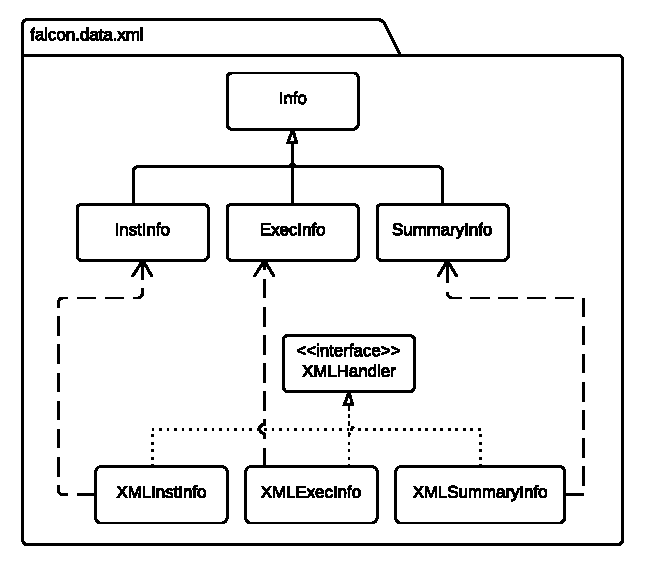
\includegraphics[width=.8\textwidth]{FalconXML.pdf}\\
  \caption{falcon.data.xml包UML类图}\label{pic:FalconXML}
\end{figure}
首先创建XMLHandler接口,包含有\texttt{Serialize(Info, path)}和\texttt{deSerialize(path)}两个方法。再分别创建XMLInstInfo、XMLExecInfo和XMLSummaryInfo 三个类来实现XMLHandler接口。\par
InstInfo类包括被调用的方法列表和程序中出现的变量构成的列表。经过序列化之后生成的instInfo.xml的片段如代码
\ref{lst:instxml}所示,XML元素的解释见表\ref{tab:instXMLele}。\\
\begin{code}[language=XML, label=lst:instxml, caption=instInfo.xml片段]
<methodInfo>
 <mid>4</mid>
 <msig>&lt;contest.account.Account: void transfer(...)&gt;</msig>
</methodInfo>
<variableInfo>
 <vid>6</vid>
 <vtype>WF</vtype>
 <vsig>this.&lt;contest.account.Account:double amount&gt;</vsig>
 <vfile>Account.java</vfile>
 <vline>24</vline>
</variableInfo>
\end{code}
\begin{table}[!ht]
    \centering
    \zihao{4}
    \caption{instInfo.xml元素介绍}\label{tab:instXMLele}
    \begin{tabular}{|l|l|}
      \hline
       XML文档元素 & 解释\\\hline
       <mid>4</mid> & 方法的编号为4\\\hline
       <msig>...</msig> & 方法的签名\\\hline
       <vid>6</vid> & 变量的编号是6\\\hline
       <vtype>WF</vtype> & 变量的操作类型是写类属性\\\hline
       <vsig>...</vsig> & 变量的签名\\\hline
       <vfile>Account.java</vfile> & 变量在Account.java文件中\\\hline
       <vline>24</vline> & 变量出现在第24行\\\hline
    \end{tabular}
\end{table}\par
ExecInfo类包含有该次程序运行的结果和出现的数据访问模式。经过序列化之后生成的execInfo.xml。SummaryInfo类包含有多次运行结果的统计信息和各个数据访问模式的信息、可疑度。其中,顺序破坏和原子性破坏这两种数据访问模式是最主要的信息。经过序列化后,这两部分信息会如代码\ref{lst:execxml}所示保存成XML文档,其中XML元素的解释见表\ref{tab:execXMLele}。\\
\begin{code}[language=XML, label=lst:execxml, caption=execInfo.xml片段]
<order>
    <pass>9</pass>
    <fail>1</fail>
    <susp>10</susp>
    <stack1></stack1>
    <stack2></stack2>
    <var1>6</var1>
    <var2>8</var2>
</order>
<atomicity>
    <pass>0</pass>
    <fail>1</fail>
    <susp>100</susp>
    <stack1></stack1>
    <stack2></stack2>
    <var1>4</var1>
    <var2>2</var2>
    <stack3></stack3>
    <var3>27</var3>
</atomicity>
\end{code}
\begin{table}[!ht]
    \centering
    \zihao{4}
    \caption{数据访问模式序列化为XML}\label{tab:execXMLele}
    \begin{tabular}{|l|l|}
      \hline
      XML文档元素 & 解释\\\hline
       <pass>9</pass> & 被测程序执行了10次,其中9次得到正确结果\\\hline
       <fail>1</fail> & 被测程序有一次运行结果错误\\\hline
       <susp>10</susp> & 可疑度是10\%\\\hline
       <var1>6</var1> & 模式的第一个操作的变量编号是6\\\hline
       <stack1></stack1> & 方法调用序列\\\hline
    \end{tabular}
\end{table}
\subsection{改进}
由于被分析的源码并不完整,需要对代码进行补充才能够运行。另外,本文以Martin Fowler的《重构——改善既有代码的设计》一书为指导,对源代码的部分实现过程进行了重构。虽然重构的操作比较琐碎,但是提高了代码的可读性,一些代码做到了复用。
\subsubsection{对源代码的补充}
被分析的源代码由于不完整,因此不能够对\texttt{startTestCase()} 和\texttt{endTestCase()}进行插装。缺少的这一部分代码涉及到了滑动窗口的初始化和返回被测程序运行结果等关键步骤,所以必须补充完整才能使Falcon运行。本文作者补充了这一部分的代码,使Falcon可以运行。此外,本文作者对Falcon 原有算法的完善主要包括两点:
\begin{enumerate}
  \item 增加了对If语句和Switch语句的分析;
  \item 增加了对含静态变量的类的处理。
\end{enumerate}
关于以上两点的具体实现,本文作者所做的工作在\ref{sec:InstProcess}中已做了具体介绍和解释。
\subsubsection{对Falcon的重构}
本次毕业设计中对原有代码的重构包括以下几点:\\
1. 封装字段\\
falcon/data/structure中部分类中public字段改为private,并且加入相应的访问函数。\\
2. 重构部分方法
\begin{itemize}
  \item 提炼函数,将过长的代码段放入独立的函数中,如添加ExecInfo类, SummaryInfo类中\texttt{print()}方法等;
  \item 以直接访问类属性取代方法调用,修改InstMethod类和InstVariable类的toString方法,减少方法调用次数,提高效率。
\end{itemize}
3. 使用Enum类型
\begin{itemize}
  \item 添加ExecuteResult枚举类,替换之前使用int类型表示运行结果;
  \item 重写EventType枚举类,添加\texttt{toString()}方法,删去\texttt{getTypeString()} 方法。
\end{itemize}
4.提炼接口\\
将用于序列化和反序列化的\texttt{Serialize()}和\texttt{deSerialize()}提炼到一个独立的接口中。\\
5.提炼超类\\
将ExecInfo、InstInfo和SummaryInfo三个类中相同的属性和方法移至超类Info中。\\
6. 修改部分代码,使满足编程规范。
\subsection{运行环境与配置}
\subsubsection{运行环境}
\noindent 硬件
\begin{itemize}
  \item CPU:Intel Core 2 Duo T6500, 2.1GHz
  \item 内存:2G
\end{itemize}
软件
\begin{itemize}
  \item Java运行环境:Java SE 1.7
  \item Python运行环境:Python3.3
  \item 开发环境:Eclipse 4.2
  \item 构建工具:Apache Ant 1.8.4
  \item 基准程序: The ConTest Benchmark Suite
  \item Soot 2.4.0\footnote{目前Soot的最新版本是2.5.0,但是使用该版本有兼容性问题。}
\end{itemize}\par
Apache Ant是一个将Java编译、测试、部署等步骤联系在一起加以自动化的一个工具,脚本格式为XML。Ant和C语言使用的make脚本一样,可以用于自动化调用程序完成项目的编译,打包,测试等。Python是一门面向对象的解释型编程语言。在Falcon当中,使用Python 脚本用来调用Ant的build文件,便于自动化运行多个被测程序。The ConTest Benchmark Suite由一组包含有并发错误的Java 多线程小程序(代码行均小于1000行)组成的基准程序,可以用来检验多线程测试工具的有效性\cite{eytani2007towards}。 ConTest Benchmark里的程序都给出了具体的场景,即预期的输出结果,这样便于判断程序的实际输出结果是否正确。程序中的错误在文档里都进行了详细的分析和说明,这样便于和错误定位工具得到的结果进行比对,从而可以检测工具的有效性。
\subsubsection{配置过程}
\begin{enumerate}
  \item 安装Eclipse插件
  \begin{itemize}
    \item Python插件PyDev\footnote{http://pydev.org/download.html}
  \end{itemize}
  \item 创建工作目录(Falcon\_Root)
  \item 创建子目录
  \begin{itemize}
    \item Falcon\_Root/falcon,用来存放Falcon代码
    \item Falcon\_Root/subjects,用来存放基准程序
    \item Falcon\_Root/library,用来存放类库
  \end{itemize}
  \item 添加需要的类库至Falcon\_Root/library
  \begin{itemize}
    \item sootclasses.jar
    \item jasminclasses.jar
    \item java\_cup.jar
    \item polyglot.jar\footnote{以上四个jar包均可以在http://www.sable.mcgill.ca/soot/soot\_download.html下载。}
    \item xpp3\_min.jar\footnote{http://mvnrepository.com/artifact/xpp3/xpp3\_min}
    \item xstream.jar\footnote{http://xstream.codehaus.org/download.html}
  \end{itemize}
  \item 导入项目代码,配置类库路径
\end{enumerate}
\subsubsection{运行}
Falcon运行的流程如图\ref{pic:FlowDiagram}所示。
\begin{figure}[!ht]
  \centering
  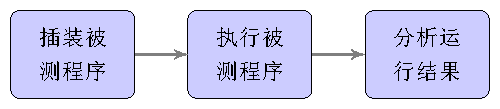
\includegraphics[width=.8\textwidth]{FlowDiagram.pdf}\\
  \caption{Falcon运行流程图}\label{pic:FlowDiagram}
\end{figure}\par
在Eclipse上运行,具体包括一下几个步骤:\\
1.编译\\
编译Falcon和Benchmark。在Eclipse中,可以直接右键build.xml选择执行ant。\\
2.插装\\
运行inst.py,调用build.xml中的inst任务进行插装。在安装过PyDev的Eclipse中,可以直接运行python脚本。\\
3.运行\\
运行exec.py,调用run.xml运行被测程序。\\
4.纠正运行结果\\
运行result.py,读取日志文件纠正execInfo.xml中错误的运行结果。\\
5.输出排序结果\\
运行output.py,调用run.xml得到统计结果。
\subsection{运行结果}
\noindent\textbf{插装结果}\par
第一步插装之后,Falcon会生成记录静态分析被测程序过程的日志文件和保存有插装结果的instInfo.xml,同时,还会得到经过插装的.class文件。\\
\textbf{运行结果}\par
第二部运行经过插装的被测程序(第一步生成的经过插装的.class文件),每运行一次被测程序,会生成带有运行结果的日志文件(.log)和保存有每一个数据访问模式的execInfo.xml。\\
\textbf{输出结果}\par
最后一步之后,Falcon会生成两个文件来保存结果,分别是序列化后的summaryInfo.xml和显示结果的rank.txt。其中rank.txt的输出结果如下所示。\\
~\\
\fbox{
\begin{minipage}{.95\textwidth}
\zihao{5}
--------------------------------------------------------\\
		Result\\
--------------------------------------------------------\\
Total Pass: 3\\
Total Fail: 7\\
Total Deadlock: 0\\
--------------------------------------------------------\\
		printing order violation\\
| rank | pass | fail | deadlock | access1 | access2 | score |\\
--------------------------------------------------------\\
| 1 | 3 | 7 | 0 | WF @Account.java:25 | WF @Account.java:26 | 70.0\% |\\
| 2 | 0 | 3 | 0 | RF @Account.java:31 | WF @Account.java:21 | 42.0\% |\\
| 3 | 0 | 3 | 0 | WF @Account.java:26 | RF @Main.java:73 | 42.0\% |\\
\ldots\\
--------------------------------------------------------\\
		printing atomicity violation\\
| rank | pass | fail | deadlock | access1 | access2 | access3 | score |\\
--------------------------------------------------------\\
| 1 | 3 | 7 | 0 | RF @Account.java:31 | WF @Account.java:25 | RF @Main.java:73 | 70.0\% |\\
| 2 | 3 | 7 | 0 | RF @Account.java:31 | WF @Account.java:26 | RF @Main.java:73 | 70.0\% |\\
| 3 | 0 | 4 | 0 | RF @Account.java:26 | WF @Account.java:25 | WF @Account.java:26 | 57.0\% |\\
| 4 | 1 | 4 | 0 | WF @Account.java:21 | WF @Account.java:26 | WF @Account.java:25 | 50.0\% |\\
| 5 | 0 | 3 | 0 | RF @Account.java:31 | WF @Account.java:25 | RF @Main.java:71 | 42.0\% |\\
| 6 | 0 | 3 | 0 | RF @Account.java:31 | WF @Account.java:26 | RF @Main.java:71 | 42.0\% |\\
\ldots\\
\end{minipage}
}\\
~\par
示例的程序是The ConTest Benchmark Suite中的一个小程序。经过插装后共运行了10遍。首先Result显示了这10次运行,一共有3次通过,剩下7次得到的结果都与预期不符,没有出现死锁。接着显示的是按照可疑度由高到低排列的顺序破坏数据访问模式。其中,排名第1 的模式是$W_1-W_2$型的顺序破坏。变量所在的位置分别是Account.java的第25行和Account.java的第26行。在10次运行中,有3次结果正确,7 次结果错误。按照公式\ref{Jaccard}可以计算出可疑度是70\%。顺序破坏数据访问模式过后,显示的是按照可疑度由高到低排列的原子性破坏数据访问模式,输出信息的具体含义与顺序破坏的相同。
